% Provenance (never printed): see sources/outline_sources.md (Year 1: vertical structure of
% the atmosphere, lapse rates, potential temperature and static stability; the layered
% ocean, the equation of state of seawater, T-S diagrams and water masses). Exercise and
% problem values in the Book 3 scratch calculator calc/ch26.py; figures from
% figdata/bachelor-1/atmosphere_profile.py (U.S. Standard Atmosphere 1976) and
% seawater_eos.py (EOS-80 and the UNESCO 44 algorithms; WOA23 columns, datasets
% bachelor-1-woa23-* and Book 2's grade-10-woa23-arctic-*).
% Physics owns the hydrostatic relation, the isothermal atmosphere and its scale height,
% the first law, Laplace's relation and Archimedes' thrust (recalled). Book 1 (g8) gave
% the layers and the environmental lapse rate of 6.5 K/km; Book 2 (g10) the dry adiabatic
% rate admitted, stable and unstable air, the mixed layer, thermocline, halocline and
% pycnocline: re-founded here with derivations. The moist adiabat is the Year 2 volume's.
\chapter{大气与海洋的结构}\label{ch:b1:fluid-envelopes-structure}

每天两次，世界各地的气象站都会放飞一只气球，
球上挂着探空仪，这是一种小型仪器，它随气球上升，把气压、温度
和湿度的数据用无线电传回地面；气球以约 \qty{300}{m} 每分钟的速度上升，
可上升至 \qty{35}{km} 才破裂。远离陆地的海上，一艘科考船
用缆绳把装有仪器和采水瓶的框架放入深海，
沿途测量电导率、温度和深度。这两条
廓线，一条为空气的，一条为海水的，是本章的原始资料。
两个圈层都是分层的，而且分层都由密度决定：
轻流体在上，重流体在下。一层是轻是重，
其实没有表面看起来那么显然。比下层空气更冷的空气，
仍可能更轻；比上层海水更暖的海水，仍可能更重。
本章将建立理清这一点的两个工具，即\omterm{def:b1:fluid-envelopes-structure:potential-temperature}{位温}
与\omterm{def:b1:fluid-envelopes-structure:eos}{海水状态方程}。
% ledger: nws:radiosonde, nws:radiosonde-def, commons:ctd-rosette

\begin{omfigure}
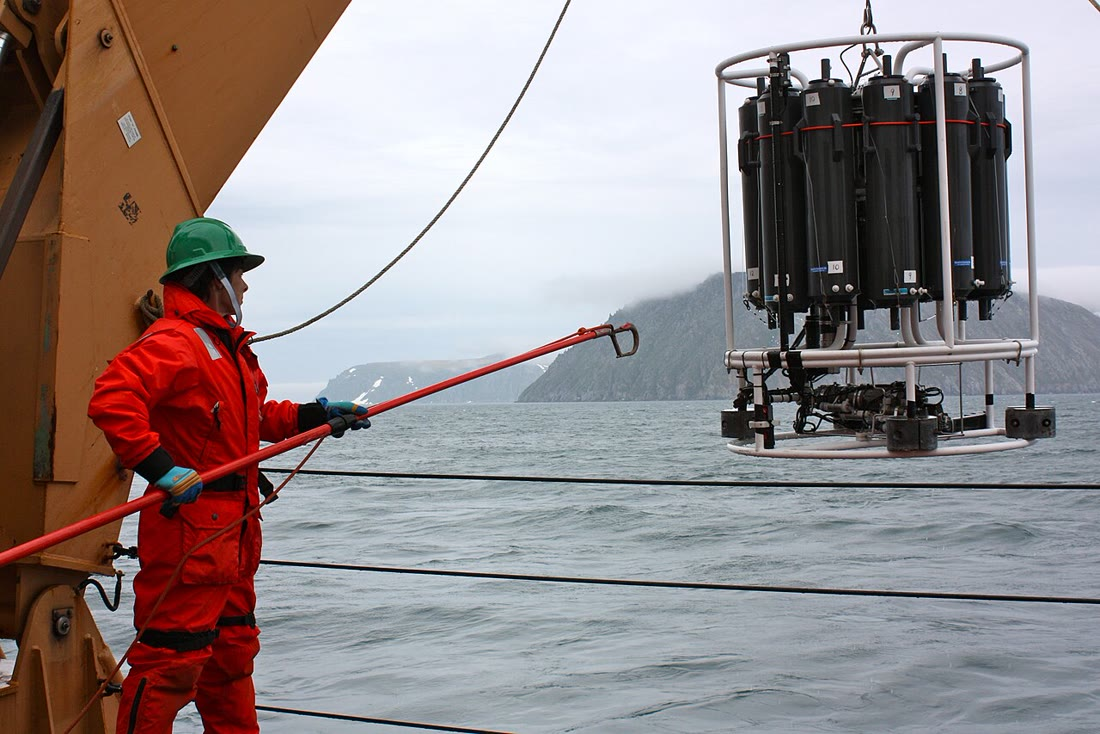
\includegraphics[width=0.62\linewidth]{images/book3/b1-ctd-rosette.jpg}

{\small 2011 年 6 月，CTD 与采水框架在白令海峡被收回船上。
框架周围的灰色采水瓶在上升途中于选定深度关闭，以采集水样；
框架底部的仪器随框架下放连续测量电导率（由此算出盐度）、
温度和深度（实际为
压强）。（NASA Goddard Space Flight
Center，公有领域，经由维基共享资源。）}
\label{fig:b1:fluid-envelopes-structure:ctd}
\end{omfigure}
% ledger: commons:ctd-rosette, unesco44:atg-theta

\begin{recall}
物理分册给出静止流体的静力学关系 $\mathrm dp/\mathrm dz =
-\rho g$；对摩尔质量为 $M$ 的理想气体，$p = \rho R
T/M$，在等温大气中气压按 $e^{-z/H}$ 随高度下降，其中
标高 $H = RT/(Mg)$。书中给出封闭系统的热力学第一定律，
以及理想气体沿可逆绝热
过程的拉普拉斯关系 $pV^{\gamma} = $ 常数，其中 $\gamma = c_p/c_v$，且 $c_p - c_v
= R/M$（按单位质量计）。浸入流体中的物体受到向上的浮力等于
它所排开流体的重量（阿基米德）。第 1 册给出了大气的各层，
以及\omterm{def:b1:fluid-envelopes-structure:standard-atmosphere}{标准大气}的\omterm{def:b1:fluid-envelopes-structure:lapse-rate}{环境递减率}，
对流层中每千米 \qty{6.5}{\celsius}；第 2 册承认了\omterm{def:b1:fluid-envelopes-structure:lapse-rate}{干绝热
递减率}为每千米 \qty{9.8}{\celsius}，依据被上推\omterm{def:b1:fluid-envelopes-structure:parcel}{气块}的去向判断空气稳定或不稳定，
并描述了海洋的\omterm{def:b1:fluid-envelopes-structure:ocean-layers}{混合层}、
\omterm{def:b1:fluid-envelopes-structure:ocean-layers}{温跃层}、\omterm{def:b1:fluid-envelopes-structure:ocean-layers}{盐跃层}和\omterm{def:b1:fluid-envelopes-structure:ocean-layers}{密度跃层}。海水的盐度
接近每千克含 35 克溶解盐。
% ledger: ussa76:layers, nws:dalr, nos:salinity
\end{recall}

\section{大气的垂直结构}\label{sec:b1:fluid-envelopes-structure:atmosphere}

没有两次实测探空彼此完全相同。为便于比较，
须按约定固定一条参考廓线。

\begin{definition}[标准大气]\label{def:b1:fluid-envelopes-structure:standard-atmosphere}
称\emph{标准大气}\index{标准大气}为温度、气压和密度随高度变化的
按约定固定的廓线：干空气
摩尔质量恒定、处于静力平衡的理想气体，海平面处给定数值，
且温度在相继各层中随高度线性变化。
1976 年标准大气在海平面取 \qty{288.15}{K} 和
\qty{101325}{Pa}，$M_0 = \qty{28.9644}{kg.kmol^{-1}}$，
$R^* = \qty{8314.32}{J.kmol^{-1}.K^{-1}}$，$g_0 = \qty{9.80665}{m.s^{-2}}$。
\end{definition}
% ledger: ussa76:sea-level

在 \qty{47}{km} 以下，1976 年\omterm{def:b1:fluid-envelopes-structure:standard-atmosphere}{标准大气}分为四层
（见\cref{tab:b1:fluid-envelopes-structure:layers}）。最低的一层是对流层，
以每千米 \qty{6.5}{K} 的速率降温；其顶为对流层顶，
温度在其上 9 千米内保持 \qty{216.65}{K} 不变，然后升高。
\omterm{def:b1:fluid-envelopes-structure:standard-atmosphere}{标准大气}中的高度是位势高度，即在恒定
重力 $g_0$ 下与之势能相同的高度；\qty{32}{km} 以下，它们与几何高度的
偏差小于 \qty{0.6}{\percent}
（\omterm{def:b1:fluid-envelopes-structure:standard-atmosphere}{标准大气}中的 \qty{11}{km} 处位于 \qty{11.02}{km}）。
% ledger: ussa76:layers, ussa76:sea-level

\begin{table}[ht]
\centering
\small
\renewcommand{\arraystretch}{1.2}
\begin{tabular}{|l|c|c|c|c|}
\hline
层 & 底部高度 (km) & $\mathrm dT/\mathrm dz$ (K/km) & 底部 $T$ (K) & 底部 $p$ (hPa) \\
\hline
1（对流层） & 0 & $-6.5$ & 288.15 & 1013.25 \\
2（平流层） & 11 & 0.0 & 216.65 & 226.32 \\
3（平流层） & 20 & $+1.0$ & 216.65 & 54.75 \\
4（平流层） & 32 & $+2.8$ & 228.65 & 8.68 \\
\hline
\end{tabular}
\caption{1976 年\omterm{def:b1:fluid-envelopes-structure:standard-atmosphere}{标准大气}最低的四层。梯度
与海平面值是定义量；各层底部的温度和气压
由它们依\cref{prop:b1:fluid-envelopes-structure:layer-pressure}算出。}
\label{tab:b1:fluid-envelopes-structure:layers}
\end{table}
% ledger: ussa76:layers, ussa76:sea-level (bases computed in figdata/bachelor-1/atmosphere_profile.py)

在每一层内，温度是高度的线性函数，因此
静力学关系可以解析积分。

\begin{proposition}[恒定梯度层中的压强]\label{prop:b1:fluid-envelopes-structure:layer-pressure}
在干空气的一层中，若 $T = T_b - L\,(z - z_b)$，其中 $L \neq 0$ 为常数，则
压强为
\[
  p = p_b \left(\frac{T}{T_b}\right)^{gM/(RL)},
\]
其中 $T_b$ 与 $p_b$ 为底部 $z_b$ 处的值。当 $L = 0$
时，压强按标高 $H = RT_b/(Mg)$ 呈指数递减。
\end{proposition}

\begin{proof}
由静力学关系与理想气体定律得 $\mathrm dp/p = -(gM/R)\,\mathrm
dz/T$。由 $\mathrm dT = -L\,\mathrm dz$，有 $\mathrm dp/p =
(gM/(RL))\,\mathrm dT/T$，积分得 $\ln(p/p_b) = (gM/(RL))
\ln(T/T_b)$。当 $L = 0$ 时，$T = T_b$，$\ln(p/p_b) = -(z - z_b)/H$，即
物理各册中的等温大气。
\end{proof}

在\omterm{def:b1:fluid-envelopes-structure:standard-atmosphere}{标准大气}的对流层中，$gM/(RL) = 9.80665 \times 28.9644 /
(8314.32 \times 0.0065) = 5.256$，在 \qty{11}{km} 处，$T = 216.65$~K：
$p = \num{101325} \times (216.65/288.15)^{5.256} = \qty{22632}{Pa}$，略低于
海平面值的四分之一。在其上方的等温层中，$H =
8314.32 \times 216.65/(28.9644 \times 9.80665) = \qty{6.34}{km}$，再向上 9
千米处，压强又降低了 $e^{9/6.34} =
4.13$ 倍，即 \qty{5475}{Pa}。由于某一高度的压强等于其上方
单位面积上方空气的重量，故\omterm{def:b1:fluid-envelopes-structure:standard-atmosphere}{标准大气}一半的质量位于
\qty{5.5}{km} 以下，九成位于 \qty{16}{km} 以下。
% ledger: ussa76:sea-level, ussa76:layers (values computed in figdata/bachelor-1/atmosphere_profile.py)

\section{递减率与位温}\label{sec:b1:fluid-envelopes-structure:lapse}

\begin{definition}[环境递减率与干绝热递减率]\label{def:b1:fluid-envelopes-structure:lapse-rate}
\emph{环境递减率}\index{环境递减率}为 $\Gamma =
-\mathrm dT/\mathrm dz$，即静止空气的温度
随高度降低的速率，正如探空测量所示。\emph{干绝热
递减率}\index{干绝热递减率} $\Gamma_d$ 为
未饱和\omterm{def:b1:fluid-envelopes-structure:parcel}{气块}被抬升时其温度的下降速率。
\end{definition}
% ledger: nws:dalr

当温度随高度降低时，递减率为正。两者
性质不同：前者描述大气在某一时刻的状态；
后者描述运动中的一团空气所经历的过程。

\begin{definition}[气块]\label{def:b1:fluid-envelopes-structure:parcel}
\emph{气块}\index{气块}是随运动被追踪的一团空气，
其尺度足够小，以至于具有单一的温度与压强，且不扰动周围的空气，
同时又足够大以保持其自身的完整性：它与外界不交换
质量，在快速位移过程中也不与外界交换热量，其
压强时刻与周围空气的压强相同。
\end{definition}

\omterm{def:b1:fluid-envelopes-structure:parcel}{气块}与热力学中的封闭系统一样，是一种理想化的模型：
下述结论对实际空气成立的程度，取决于其中运动的一部分
与外界交换的热量与质量是否很少。

\begin{theorem}[干绝热递减率]\label{thm:b1:fluid-envelopes-structure:dry-adiabatic}
干空气\omterm{def:b1:fluid-envelopes-structure:parcel}{气块}经绝热可逆抬升，穿过温度
几乎相同的静止空气时，以下述速率降温：
\[
  \Gamma_d = \frac{g}{c_p},
\]
其中 $c_p$ 为空气的定压比热容。取 $c_p =
\qty{1004.7}{J.kg^{-1}.K^{-1}}$，则 $\Gamma_d = \qty{9.76}{K.km^{-1}}$。
\end{theorem}

\begin{proof}
对于温度为 $T_p$、密度为 $\rho_p$ 的一千克\omterm{def:b1:fluid-envelopes-structure:parcel}{气块}，
可逆、无热交换的过程的热力学第一定律，以焓的形式写出，
即 $c_p\,\mathrm dT_p - \mathrm dp/\rho_p = 0$。\omterm{def:b1:fluid-envelopes-structure:parcel}{气块}的压强
与周围空气的压强相同，而后者满足静力学关系：$\mathrm dp = -\rho_e
g\,\mathrm dz$，其中 $\rho_e$ 为周围空气的密度。于是
\[
  \frac{\mathrm dT_p}{\mathrm dz} = -\frac{g}{c_p}\,\frac{\rho_e}{\rho_p}
  = -\frac{g}{c_p}\,\frac{T_p}{T_e},
\]
由于在相同压强下，摩尔质量相同的两种理想气体的密度
与其温度成反比。当\omterm{def:b1:fluid-envelopes-structure:parcel}{气块}的温度
与周围空气温度接近时，$T_p/T_e \approx 1$，且 $-\mathrm dT_p/\mathrm dz
= g/c_p$。干空气为理想双原子气体，$\gamma = 1.4$，故 $c_p =
\gamma/(\gamma - 1) \times R/M = 3.5 \times 8314.32/28.9644 =
\qty{1004.7}{J.kg^{-1}.K^{-1}}$，且 $\Gamma_d = 9.80665/1004.7 =
\qty{0.00976}{K.m^{-1}}$.
\end{proof}
% ledger: nasa:grc-gamma, ussa76:sea-level, nws:dalr

比周围空气高 \qty{10}{K} 的\omterm{def:b1:fluid-envelopes-structure:parcel}{气块}，在 \qty{280}{K} 附近，
以 $\Gamma_d \times 290/280$ 的速率降温，快 \qty{3.6}{\percent}；此修正
在下文中略去。该速率与\omterm{def:b1:fluid-envelopes-structure:parcel}{气块}的压强或
温度无关，下沉的\omterm{def:b1:fluid-envelopes-structure:parcel}{气块}以相同速率升温，
正如第 2 册中追踪空气越山时所做的那样。

若不利用静力学一步而对同一方程积分，
可得一个随\omterm{def:b1:fluid-envelopes-structure:parcel}{气块}一同保持不变的量。

\begin{proposition}[位温]\label{prop:b1:fluid-envelopes-structure:theta}
沿干空气的可逆绝热过程，
\[
  \theta = T\left(\frac{p_0}{p}\right)^{\kappa},\qquad \kappa = \frac{R}{Mc_p} =
  \frac{\gamma - 1}{\gamma} = \frac{2}{7},
\]
保持不变，与参考压强 $p_0$ 的选取无关。
\end{proposition}

\begin{proof}
由 $c_p\,\mathrm dT = \mathrm dp/\rho$ 及 $\rho = pM/(RT)$，得 $c_p\,\mathrm dT/T
= (R/M)\,\mathrm dp/p$，故 $\ln T - \kappa \ln p$ 为常数，$T
p^{-\kappa}$ 亦然；乘以常数 $p_0^{\kappa}$ 即得 $\theta$。此即
以 $T$ 与 $p$ 写出的拉普拉斯关系。
\end{proof}

\begin{definition}[位温]\label{def:b1:fluid-envelopes-structure:potential-temperature}
干空\omterm{def:b1:fluid-envelopes-structure:parcel}{气块}的\emph{位温}\index{位温}$\theta$，是将其绝热地调整至
参考压强 $p_0 = \qty{1000}{hPa}$ 时所具有的温度，
即 $\theta = T\,(1000/p)^{2/7}$，其中 $p$ 以百帕为单位，
$T$ 以开尔文为单位。
\end{definition}
% ledger: nws:potential-temperature

\omterm{def:b1:fluid-envelopes-structure:potential-temperature}{位温}是干空\omterm{def:b1:fluid-envelopes-structure:parcel}{气块}在上升或下沉且不与外界交换热量时保持不变的量，
正如\omterm{def:b1:fluid-envelopes-structure:ts-diagram}{水团}的盐度。辐射加热、水汽凝结或混合会改变它；
其余过程则不会。

\begin{example}[标准大气的对流层顶]\label{ex:b1:fluid-envelopes-structure:tropopause}
在\omterm{def:b1:fluid-envelopes-structure:standard-atmosphere}{标准大气}的地面处，$\theta = 288.15 \times (1000/1013.25)^{2/7} =
\qty{287.07}{K}$。在对流层顶，$T = \qty{216.65}{K}$，$p =
\qty{226.32}{hPa}$：$\theta = 216.65 \times (1000/226.32)^{2/7} = 216.65 \times
1.529 = \qty{331.2}{K}$。将对流层顶的空气绝热下沉至
\qty{1000}{hPa}，其温度将达到 \qty{331.2}{K}，比同一压强下的
地面空气高出 \qty{44}{K}。从地面到对流层顶，温度下降了 \qty{71.5}{K}，
而\omterm{def:b1:fluid-envelopes-structure:potential-temperature}{位温}却上升了
\qty{44}{K}。
\end{example}
% ledger: ussa76:layers, nws:potential-temperature (values computed in figdata/bachelor-1/atmosphere_profile.py)

\section{静力稳定度}\label{sec:b1:fluid-envelopes-structure:stability}

\begin{definition}[静力稳定度；逆温]\label{def:b1:fluid-envelopes-structure:stability}
静止层的\emph{静力稳定度}\index{静力稳定度}，是其对
\omterm{def:b1:fluid-envelopes-structure:parcel}{气块}微小竖直位移的响应。若位移后的\omterm{def:b1:fluid-envelopes-structure:parcel}{气块}被推回其原高度，则该层具有
\emph{稳定层结}\index{稳定层结}；若被推得更远，则具有
\emph{不稳定层结}\index{不稳定层结}；若不受任何力作用，则具有
\emph{中性层结}\index{中性层结}。
\emph{逆温}\index{逆温}是指
温度随高度增加的
一层。
\end{definition}
% ledger: nws:inversion

\begin{theorem}[静力稳定判据]\label{thm:b1:fluid-envelopes-structure:stability}
设静止干空气层的温度为 $T$，\omterm{def:b1:fluid-envelopes-structure:lapse-rate}{环境递减率}为
$\Gamma$，则当 $\Gamma < \Gamma_d$ 时该层稳定，$\Gamma = \Gamma_d$ 时中性，
$\Gamma > \Gamma_d$ 时不稳定；等价地，当且仅当其
\omterm{def:b1:fluid-envelopes-structure:potential-temperature}{位温}随高度增加时该层稳定。被微小位移
$\delta z$ 的\omterm{def:b1:fluid-envelopes-structure:parcel}{气块}绕其所在高度振荡，角频率为
$N$，其中
\[
  N^2 = \frac{g}{T}\,(\Gamma_d - \Gamma) = \frac{g}{\theta}\,\frac{\mathrm d\theta}{\mathrm dz}.
\]
\end{theorem}

\begin{proof}
\omterm{def:b1:fluid-envelopes-structure:parcel}{气块}位于其所在高度的温度 $T$ 处，被抬升 $\delta z$。它
到达的温度为 $T - \Gamma_d\,\delta z$，而周围空气的温度为 $T - \Gamma\,\delta z$。
单位质量的\omterm{def:b1:fluid-envelopes-structure:parcel}{气块}受到重力与阿基米德浮力的作用，
竖直向上的净加速度为 $g\,(\rho_e - \rho_p)/\rho_p = g\,(T_p - T_e)/T_e$，
两者压强相等。取 $\delta z$ 的一阶近似，有
\[
  \frac{\mathrm d^2 \delta z}{\mathrm dt^2} = -\frac{g}{T}\,(\Gamma_d - \Gamma)\,\delta z = -N^2\,\delta z .
\]
若 $\Gamma < \Gamma_d$，则 $N^2 > 0$，\omterm{def:b1:fluid-envelopes-structure:parcel}{气块}以角频率
$N$ 振荡；若 $\Gamma > \Gamma_d$，位移呈指数增长；若
$\Gamma = \Gamma_d$，则不受任何力作用。对于第二种形式，取
$\theta = T (p_0/p)^{\kappa}$ 的对数导数，并利用静力平衡关系：
\[
  \frac{1}{\theta}\frac{\mathrm d\theta}{\mathrm dz} = \frac{1}{T}\frac{\mathrm dT}{\mathrm dz}
  - \frac{\kappa}{p}\frac{\mathrm dp}{\mathrm dz} = -\frac{\Gamma}{T} + \frac{\kappa\,\rho g}{p}
  = -\frac{\Gamma}{T} + \frac{\kappa g M}{RT} = \frac{\Gamma_d - \Gamma}{T},
\]
由于 $\kappa M/R = 1/c_p$。
\end{proof}

角频率 $N$ 称为浮力频率。在\omterm{def:b1:fluid-envelopes-structure:standard-atmosphere}{标准大气}的
对流层中、靠近地面处，$N^2 = (9.80665/288.15) \times (9.761 -
6.5)\times10^{-3} = \qty{1.11e-4}{s^{-2}}$，$N = \qty{0.0105}{s^{-1}}$，
振荡周期 $2\pi/N$ 约为 \qty{10}{min}。在等温的
下平流层中 $\Gamma = 0$：$N = \qty{0.0210}{s^{-1}}$，为前者的两倍，
周期为五分钟。平流层像一个盖子：它对竖直运动的抑制
远强于其下方的对流层。
% ledger: ussa76:layers (values computed in figdata/bachelor-1/atmosphere_profile.py)

\begin{omfigure}
\begin{tikzpicture}
\begin{axis}[name=tz, omrecord, width=0.46\linewidth, height=7.2cm, xmin=160, xmax=300,
  ymin=0, ymax=32, xlabel={温度 (K)}, ylabel={高度 (km)}, xtick={160,200,...,300},
  ytick={0,5,...,30}]
% figdata/bachelor-1/atmosphere_profile.py; ledger: ussa76:sea-level, ussa76:layers, nasa:grc-gamma
\addplot[omDef, line width=0.9pt] table[x=T_K, y=z_km] {figdata/out/bachelor-1-atmosphere_profile-profile.dat};
\addplot[omThm, dashed, line width=0.7pt] table[x=T_K, y=z_km] {figdata/out/bachelor-1-atmosphere_profile-adiabat.dat};
\addplot[only marks, mark=*, mark size=1.6pt, black] table[x=T_K, y=z_km] {figdata/out/bachelor-1-atmosphere_profile-tropo.dat};
\node[font=\scriptsize, text=omThm, anchor=west, align=left] at (axis cs:163,17.0) {从地面出发的 \\干绝热线};
\node[font=\scriptsize, text=omDef, anchor=west] at (axis cs:252,6.4) {标准大气};
\node[font=\scriptsize, anchor=east] at (axis cs:214.5,11.9) {对流层顶};
\end{axis}
\begin{axis}[at={(tz.east)}, anchor=west, xshift=1.3cm, omrecord, width=0.46\linewidth, height=7.2cm,
  xmin=250, xmax=900, ymin=0, ymax=32, xlabel={位温 (K)}, ylabel={高度 (km)},
  xtick={300,500,700,900}, ytick={0,5,...,30}]
\addplot[omDef, line width=0.9pt] table[x=theta_K, y=z_km] {figdata/out/bachelor-1-atmosphere_profile-profile.dat};
\addplot[only marks, mark=*, mark size=1.6pt, black] table[x=theta_K, y=z_km] {figdata/out/bachelor-1-atmosphere_profile-tropo.dat};
\node[font=\scriptsize, anchor=west] at (axis cs:345,10.2) {\num{331} K};
\end{axis}
\end{tikzpicture}

{\small 1976 年\omterm{def:b1:fluid-envelopes-structure:standard-atmosphere}{标准大气}至 \qty{32}{km}。左：温度，并给出从地面抬升的\omterm{def:b1:fluid-envelopes-structure:parcel}{气块}
所遵循的干绝热线（虚线）。\omterm{def:b1:fluid-envelopes-structure:standard-atmosphere}{标准大气}的降温比绝热线慢，因此处处稳定。
右：\omterm{def:b1:fluid-envelopes-structure:potential-temperature}{位温}，
它随高度处处增加，在对流层中增加缓慢，
在对流层顶以上则迅速增加（圆点）。}
\label{fig:b1:fluid-envelopes-structure:theta}
\end{omfigure}
% ledger: ussa76:sea-level, ussa76:layers, nasa:grc-gamma, nws:potential-temperature

在温度对高度的图上，判据比较两条线的斜率
（见下图）：\omterm{def:b1:fluid-envelopes-structure:parcel}{气块}沿经过其出发点的干绝热线变化，
关键在于，\omterm{def:b1:fluid-envelopes-structure:parcel}{气块}经过一个微小位移之后，
位于探测曲线的哪一侧。

\begin{omfigure}
\begin{tikzpicture}[x=0.55cm, y=0.55cm, >={Stealth[length=2mm]}]
\foreach \dx/\envtop/\verdict in {0/-0.8/{稳定层：气块沉回原处}, 9/-3.8/{不稳定层：气块继续上升}} {
  \begin{scope}[xshift=\dx cm]
  \draw[->] (0,0) -- (7.2,0) node[below left, font=\scriptsize] {温度};
  \draw[->] (0,0) -- (0,6.4) node[above right, font=\scriptsize] {高度};
  % sounding (environment): solid; dry adiabat through the starting point P: dashed
  \draw[omDef, line width=0.9pt] (5.0,0.6) -- (5.0+\envtop,5.4);
  \draw[omThm, dashed, line width=0.8pt] (5.0,0.6) -- (2.6,5.4);
  \fill (5.0,0.6) circle (2pt) node[right, font=\scriptsize] {$P$};
  \draw[densely dotted] (0,4.2) node[left, font=\scriptsize] {$z + \delta z$} -- (7,4.2);
  \fill[omThm] (3.2,4.2) circle (1.8pt);
  \fill[omDef] ({5.0+\envtop*3.6/4.8},4.2) circle (1.8pt);
  \node[font=\scriptsize, anchor=north] at (3.6,-0.5) {\verdict};
  \end{scope}
}
\end{tikzpicture}

{\small \omterm{def:b1:fluid-envelopes-structure:parcel}{气块}法。实线（蓝色）：探测曲线；虚线（红色）：
经过 $P$ 的干绝热线。\omterm{def:b1:fluid-envelopes-structure:parcel}{气块}从 $P$ 出发，温度与周围空气相同，
沿干绝热线被抬升到 $z + \delta z$（红色圆点）；
探测曲线给出该处空气的温度（蓝色圆点）。左：探测曲线降温
比绝热线慢，\omterm{def:b1:fluid-envelopes-structure:parcel}{气块}到达时比周围空气更冷、因而更重，于是下沉回落。
右：探测曲线降温比绝热线快，\omterm{def:b1:fluid-envelopes-structure:parcel}{气块}到达时比周围空气更暖，
于是继续上升。}
\label{fig:b1:fluid-envelopes-structure:parcel}
\end{omfigure}

\begin{method}[读取探测曲线的稳定性]\label{met:b1:fluid-envelopes-structure:sounding}
\begin{enumerate}
  \item 在斜率发生变化的高度之间，将探测曲线分成若干层。
  \item 对每一层计算 $\Gamma = -(T_2 - T_1)/(z_2 - z_1)$，单位为开尔文每
        千米。
  \item 与 $\Gamma_d = \qty{9.8}{K/km}$ 比较：$\Gamma > \Gamma_d$ 为不稳定，
        $\Gamma$ 接近 $\Gamma_d$ 为中性，$\Gamma < \Gamma_d$ 为稳定；
        $\Gamma$ 为负即为\omterm{def:b1:fluid-envelopes-structure:stability}{逆温}，是最稳定的情形。
  \item 若给出的是气压而非高度，则在各层按 $\theta =
        T(1000/p)^{2/7}$ 计算\omterm{def:b1:fluid-envelopes-structure:potential-temperature}{位温}：$\theta$ 随高度减小表示不稳定层，
        不变表示中性层，增大表示稳定层。
\end{enumerate}
\end{method}

不稳定层不会持久：其中的位移按指数规律增长，
增长速率为 $\sqrt{-N^2}$，其释放的\omterm{def:b1:fluid-envelopes-structure:parcel}{气块}使之翻转并混合，直至
\omterm{def:b1:fluid-envelopes-structure:potential-temperature}{位温}均匀、递减率等于 $\Gamma_d$。
从下方受热（如温暖的地面或海面）的层趋于不稳定，
从下方受冷的层则趋于稳定。\omterm{def:b1:fluid-envelopes-structure:stability}{逆温}层覆盖其下方的一切：自下方上升
的\omterm{def:b1:fluid-envelopes-structure:parcel}{气块}一进入\omterm{def:b1:fluid-envelopes-structure:stability}{逆温}层，便比周围空气更冷。
\omterm{def:b1:fluid-envelopes-structure:standard-atmosphere}{标准大气}在 \qty{20}{km} 以上的整个平流层
都是\omterm{def:b1:fluid-envelopes-structure:stability}{逆温}层。

以上讨论均假定空气干燥。上升的\omterm{def:b1:fluid-envelopes-structure:parcel}{气块}若达到饱和，
其中水汽凝结时释放潜热，降温便比 $\Gamma_d$ 慢；
饱和绝热线及由此带来的条件性不稳定，
将在本科二年级分册中讨论。
% ledger: nws:inversion, nws:dalr

\section{分层的海洋}\label{sec:b1:fluid-envelopes-structure:ocean}

海洋仅通过其表面与大气交换热量和水分，
方式包括加热与冷却、蒸发和降雨。其垂直结构
由温度、盐度和密度三个要素构成。

\begin{definition}[混合层、温跃层、盐跃层、密度跃层]\label{def:b1:fluid-envelopes-structure:ocean-layers}
\emph{混合层}\index{混合层}是海洋的表层，
其温度、盐度和密度几乎不随深度变化；
在剖面上，其深度读作温度首次与表层值
相差达到选定阈值处的深度，阈值常取 \qty{0.5}{\celsius}。
\emph{温跃层}\index{温跃层}、\emph{盐跃层}\index{盐跃层}和
\emph{密度跃层}\index{密度跃层}是其下方的各层，
分别是温度、盐度和密度随深度
变化最快的层。
\end{definition}

海洋中的压强以分巴为单位给出，因为一分巴
\qty{e4}{Pa}，约等于一米海水的压强：在
\qty{30}{\degree} \omterm{def:b1:spherical-astronomy:geographic}{纬度}处，\qty{1000}{dbar} 对应 \qty{990.8}{m}，
\qty{10000}{dbar} 对应 \qty{9712.7}{m}。
% ledger: unesco:eos80-checks (DEPTH table computed in figdata/bachelor-1/seawater_eos.py)

海水几乎不可压缩，但并非完全不可压缩，从深处被带到上方的
一团水与空\omterm{def:b1:fluid-envelopes-structure:parcel}{气块}一样会膨胀、降温，只是降温幅度很小。海水的
绝热递减率很小：在表面、\qty{0}{\celsius} 时，每
\qty{1000}{dbar} 约降低 \qty{0.04}{\celsius}；在 \qty{3000}{dbar} 处，
每 \qty{1000}{dbar} 约降低 \qty{0.09}{\celsius}，而空气中每千米降低
\num{9.8} 度。但在五千米的深度上，累计降温可达零点几度，
超过深层水体之间的温差。因此，海洋学家也用\emph{\omterm{def:b1:fluid-envelopes-structure:potential-temperature}{位温}}比较水体：
某一\omterm{def:b1:fluid-envelopes-structure:ts-diagram}{水团}若绝热地、在盐度不变的情况下提升至表面，
它所具有的温度即为其\omterm{def:b1:fluid-envelopes-structure:potential-temperature}{位温}。例如，\qty{4000}{dbar} 处、
\qty{2}{\celsius}、盐度为 35 的水，其\omterm{def:b1:fluid-envelopes-structure:potential-temperature}{位温}为 \qty{1.66}{\celsius}。
在南大西洋 \qty{10.5}{\degree S} 的最深层中，实测温度从
\qty{5400}{m} 处的 \qty{0.730}{\celsius} 升至
\qty{5500}{m} 处的 \qty{0.731}{\celsius}，
而\omterm{def:b1:fluid-envelopes-structure:potential-temperature}{位温}却从 \qty{0.261}{\celsius} 降至 \qty{0.250}{\celsius}：
这里的增温来自压缩，而非热量。
% ledger: unesco44:atg-theta, data:b3-woa23 (values computed in figdata/bachelor-1/seawater_eos.py)

\begin{omfigure}
\begin{tikzpicture}
\begin{groupplot}[group style={group size=3 by 1, horizontal sep=0.55cm, yticklabels at=edge left},
  omrecord, omdepth, width=0.365\linewidth, height=7.4cm, ymin=0, ymax=2000,
  ytick={0,500,1000,1500,2000}, y tick label style={/pgf/number format/.cd, set thousands separator={}},
  every axis label/.append style={font=\small}]
\nextgroupplot[xmin=-2, xmax=28, xlabel={$\theta$ (\si{\celsius})}, ylabel={深度 (m)}, xtick={0,10,20}]
% figdata/bachelor-1/seawater_eos.py; WOA23 (datasets bachelor-1-woa23-*, grade-10-woa23-arctic-*); ledger: data:b3-woa23, data:b2-woa23, unesco44:atg-theta
\addplot[omThm, line width=0.8pt] table[x=theta, y=depth] {figdata/out/bachelor-1-seawater_eos-prof-sa10.dat};
\addplot[omProp, line width=0.8pt] table[x=theta, y=depth] {figdata/out/bachelor-1-seawater_eos-prof-sa30.dat};
\addplot[omDef, line width=0.8pt] table[x=theta, y=depth] {figdata/out/bachelor-1-seawater_eos-prof-arctic.dat};
\draw[omThm, line width=0.8pt] (axis cs:9,1250) -- (axis cs:13,1250) node[right, font=\scriptsize, text=black] {\qty{10.5}{\degree S}};
\draw[omProp, line width=0.8pt] (axis cs:9,1450) -- (axis cs:13,1450) node[right, font=\scriptsize, text=black] {\qty{30.5}{\degree S}};
\draw[omDef, line width=0.8pt] (axis cs:9,1650) -- (axis cs:13,1650) node[right, font=\scriptsize, text=black] {\qty{75.5}{\degree N}};
\nextgroupplot[xmin=28, xmax=37.5, xlabel={盐度}, xtick={28,31,34,37}]
\addplot[omThm, line width=0.8pt] table[x=s, y=depth] {figdata/out/bachelor-1-seawater_eos-prof-sa10.dat};
\addplot[omProp, line width=0.8pt] table[x=s, y=depth] {figdata/out/bachelor-1-seawater_eos-prof-sa30.dat};
\addplot[omDef, line width=0.8pt] table[x=s, y=depth] {figdata/out/bachelor-1-seawater_eos-prof-arctic.dat};
\nextgroupplot[xmin=22, xmax=28.5, xlabel={$\sigma_\theta$ (\si{kg.m^{-3}})}, xtick={22,24,26,28}]
\addplot[omThm, line width=0.8pt] table[x=sigma, y=depth] {figdata/out/bachelor-1-seawater_eos-prof-sa10.dat};
\addplot[omProp, line width=0.8pt] table[x=sigma, y=depth] {figdata/out/bachelor-1-seawater_eos-prof-sa30.dat};
\addplot[omDef, line width=0.8pt] table[x=sigma, y=depth] {figdata/out/bachelor-1-seawater_eos-prof-arctic.dat};
\end{groupplot}
\end{tikzpicture}

{\small \omterm{def:b1:fluid-envelopes-structure:potential-temperature}{位温}、盐度与位\omterm{def:b1:fluid-envelopes-structure:eos}{密度异常}
（见\cref{def:b1:fluid-envelopes-structure:eos}）上层 \qty{2000}{m} 内的
年平均值，三个地点分别为热带南大西洋（\qty{10.5}{\degree
S}, \qty{25.5}{\degree W}），亚热带南大西洋（\qty{30.5}{\degree
S}, \qty{25.5}{\degree W}）与北冰洋加拿大海盆
（\qty{75.5}{\degree N}，\qty{150.5}{\degree W}）。数据：World Ocean Atlas 2023。}
\label{fig:b1:fluid-envelopes-structure:profiles}
\end{omfigure}
% ledger: data:b3-woa23, data:b2-woa23, unesco:eos80, unesco44:atg-theta

上图的三列分别代表三种上层海洋。在
热带，温暖的\omterm{def:b1:fluid-envelopes-structure:ocean-layers}{混合层}位于 \qty{26.5}{\celsius} 附近，其下为一层陡峭的
\omterm{def:b1:fluid-envelopes-structure:ocean-layers}{温跃层}：在 \qty{100}{m} 与 \qty{200}{m} 之间，\omterm{def:b1:fluid-envelopes-structure:potential-temperature}{位温}
由 \qty{24.0}{\celsius} 降至 \qty{14.4}{\celsius}，密度随之变化，
因此\omterm{def:b1:fluid-envelopes-structure:ocean-layers}{温跃层}同时也是\omterm{def:b1:fluid-envelopes-structure:ocean-layers}{密度跃层}。在 \qty{30.5}{\degree S} 处，
表层水温较低，为 \qty{21.1}{\celsius}，下降更为平缓，分布在
上层 \qty{800}{m} 之中。两者中，盐度在表层最高，
并向下递减；它对层结的作用与之相反，而温度的作用
足以将其抵消有余。北冰洋的剖面
情况恰好相反。其表层水温为 \qty{-1.4}{\celsius}，是三者中最冷的，
却也是最轻的，$\sigma_\theta = 22.5$，原因是其盐度
仅为 \num{28.1}；盐度在 \qty{300}{m} 处升至 \num{34.5}。此处的\omterm{def:b1:fluid-envelopes-structure:ocean-layers}{盐跃层}即为
\omterm{def:b1:fluid-envelopes-structure:ocean-layers}{密度跃层}。其下方是一层比上层水更暖的水，温度约为
\qty{0.7}{\celsius}，位于 \qty{475}{m} 处：这是一种完全
稳定的\omterm{def:b1:fluid-envelopes-structure:stability}{逆温}，由其盐分压住。
% ledger: data:b3-woa23, data:b2-woa23 (values computed in figdata/bachelor-1/seawater_eos.py)

\section{海水密度与温盐图}\label{sec:b1:fluid-envelopes-structure:ts}

\begin{definition}[海水状态方程；盐收缩系数；密度异常]\label{def:b1:fluid-envelopes-structure:eos}
\emph{海水状态方程}\index{海水状态方程}
给出其密度 $\rho(S, T, p)$，即盐度、温度与压强的函数。
\emph{盐收缩系数}\index{盐收缩系数}
为 $\beta = (1/\rho)\,\partial\rho/\partial S$，
温度和压强保持不变。\emph{密度异常}\index{密度异常}
$\sigma$ 为密度减去 \qty{1000}{kg.m^{-3}}：$\sigma_t = \rho(S, T, 0) -
1000$ 采用实测温度与零海压，而位密度异常
$\sigma_\theta = \rho(S, \theta, 0) - 1000$ 则采用
\omterm{def:b1:fluid-envelopes-structure:potential-temperature}{位温}。
\end{definition}
% ledger: teos10:alpha-beta, teos10:sigma

状态方程并非由第一性原理推导，而是拟合于
实验室测量数据。1980 年的国际状态方程在
表面压强下为一个含十五个系数的多项式，$\rho = \rho_w(T) +
A(T)\,S + B(T)\,S^{3/2} + C\,S^2$，其中 $\rho_w$ 为纯水的密度；
由此得 $\rho(35, \qty{0}{\celsius}) = \qty{1028.1063}{kg.m^{-3}}$。
2009 年，海水的热力学描述 TEOS-10 被采纳，以取代它
作为正式标准；本文采用 1980 年方程，因其多项式
可以写在一页之内。其热
膨胀系数 $\alpha = -(1/\rho)\,\partial\rho/\partial T$ 即
物理分册中所用的系数。
% ledger: unesco:eos80, teos10:alpha-beta, teos10:replaced

\begin{table}[ht]
\centering
\small
\renewcommand{\arraystretch}{1.2}
\begin{tabular}{|c|c|c|c|}
\hline
$T$ (\si{\celsius}) & $\rho(35, T, 0)$ (\si{kg.m^{-3}}) & $\alpha$ (\si{K^{-1}}) & $\beta$ \\
\hline
0 & 1028.106 & \num{0.53e-4} & \num{7.85e-4} \\
10 & 1026.952 & \num{1.67e-4} & \num{7.61e-4} \\
25 & 1023.343 & \num{2.97e-4} & \num{7.39e-4} \\
\hline
\end{tabular}
\caption{盐度为 35 的海水在
表面压强下的密度与膨胀系数，由 1980 年国际状态方程给出。}
\label{tab:b1:fluid-envelopes-structure:density}
\end{table}
% ledger: unesco:eos80 (computed in figdata/bachelor-1/seawater_eos.py)

热膨胀系数在温水中约为接近
凝固点的水的六倍，而 $\beta$ 几乎不变（见\cref{tab:b1:fluid-envelopes-structure:density}）。
盐度每变化一个单位，其密度效应在
\qty{10}{\celsius} 时约相当于 \qty{4.6}{\celsius} 的温度变化，而在 \qty{0}{\celsius} 附近则相当于 \qty{15}{\celsius} 的温度变化：
在寒冷的极地海水中，密度由盐度决定，如北冰洋剖面所示。

\begin{proposition}[线性状态方程]\label{prop:b1:fluid-envelopes-structure:linear-eos}
在参考状态 $(S_0, T_0)$ 附近，其密度为 $\rho_0$，压强固定时，
\[
  \rho \approx \rho_0\bigl[1 - \alpha\,(T - T_0) + \beta\,(S - S_0)\bigr],
\]
其中 $\alpha$ 与 $\beta$ 取参考状态处的值；误差为关于
$T - T_0$ 与 $S - S_0$ 的二阶小量。
\end{proposition}

\begin{proof}
这是 $\rho(S, T)$ 在 $(S_0, T_0)$ 处的一阶泰勒展开，因为
$\partial\rho/\partial T = -\rho_0\alpha$ 与 $\partial\rho/\partial S =
\rho_0\beta$ 在该处成立。
\end{proof}

在 $(35, \qty{10}{\celsius})$ 附近，线性形式给出的水体密度在
$(35.2, \qty{11}{\celsius})$ 处误差在 \qty{0.01}{kg.m^{-3}} 以内，而表层水
$(35.8, \qty{22.4}{\celsius})$ 处的密度则偏高 \qty{0.74}{kg.m^{-3}}：
状态方程是弯曲的，其曲率会产生重要后果。
% ledger: unesco:eos80 (computed in calc/ch26.py)

\begin{definition}[温盐图；水团]\label{def:b1:fluid-envelopes-structure:ts-diagram}
称\emph{温盐图}\index{温盐图}为
剖面各样品的\omterm{def:b1:fluid-envelopes-structure:potential-temperature}{位温}对其盐度所作的图，
图中沿曲线标注各深度，并在曲线下方画出等 $\sigma_\theta$ 线。
称\emph{水团}\index{水团}为具有共同形成历史的
水体，可由其\omterm{def:b1:fluid-envelopes-structure:potential-temperature}{位温}与盐度的范围加以识别。
\end{definition}
% ledger: tomczak:water-masses

\omterm{def:b1:fluid-envelopes-structure:ts-diagram}{水团}的温度与盐度在表层获得，途径为
加热与冷却、蒸发与降雨，发生于其形成的区域；一旦
\omterm{def:b1:fluid-envelopes-structure:ts-diagram}{水团}下沉至\omterm{def:b1:fluid-envelopes-structure:ocean-layers}{混合层}以下、与大气隔绝，便只能
通过与邻近水体混合来改变它们。\omterm{def:b1:fluid-envelopes-structure:potential-temperature}{位温}与盐度
此时便成为示踪剂。

\begin{proposition}[混合线是直线]\label{prop:b1:fluid-envelopes-structure:mixing}
当质量分别为 $m_1$ 和 $m_2$ 的两种水体 $(S_1, \theta_1)$ 与 $(S_2, \theta_2)$
充分混合时，混合水体满足
\[
  S = \frac{m_1 S_1 + m_2 S_2}{m_1 + m_2},\qquad
  \theta \approx \frac{m_1 \theta_1 + m_2 \theta_2}{m_1 + m_2}:
\]
在 T--S 图上，混合水体位于连接两种水体的线段上，
与两者的距离之比为其质量之比的倒数。三种水体的混合物充满
它们所围成的三角形。
\end{proposition}

\begin{proof}
盐度是盐的质量分数，盐是守恒的：混合物中盐的
质量为 $m_1 S_1 + m_2 S_2$，除以混合物质量即得 $S$。等压混合时
焓守恒；比热变化不大时，
这便是\omterm{def:b1:fluid-envelopes-structure:potential-temperature}{位温}的加权平均，相对误差在
每单位盐度差约 $3.4\times10^{-4}$ 以内。
点 $(S, \theta)$ 即为两点的重心，权重分别为
$m_1$ 与 $m_2$。
\end{proof}
% ledger: teos10:mixing

\begin{omfigure}
\begin{tikzpicture}
\begin{axis}[omrecord, width=0.82\linewidth, height=9cm, xmin=33.5, xmax=37.4, ymin=-2, ymax=28,
  xlabel={盐度}, ylabel={位温（\si{\celsius}）}, xtick={34,35,36,37},
  ytick={0,5,...,25}, x tick label style={/pgf/number format/.cd, fixed, precision=1}]
% figdata/bachelor-1/seawater_eos.py; ledger: unesco:eos80, unesco44:atg-theta, data:b3-woa23, tomczak:water-masses
\foreach \s in {24,25,26,26.5,27,27.5,28} {
  \addplot[black!35, line width=0.4pt] table[x=s, y=theta] {figdata/out/bachelor-1-seawater_eos-iso-\s.dat};
}
\addplot[only marks, mark=none, nodes near coords, point meta=explicit symbolic,
  every node near coord/.style={font=\scriptsize, text=black!55, anchor=west}]
  table[x=s, y=theta, meta=lab] {figdata/out/bachelor-1-seawater_eos-isolab.dat};
\addplot[omThm, line width=0.9pt] table[x=s, y=theta] {figdata/out/bachelor-1-seawater_eos-ts-sa10.dat};
\addplot[omProp, line width=0.9pt] table[x=s, y=theta] {figdata/out/bachelor-1-seawater_eos-ts-sa30.dat};
\addplot[only marks, mark=*, mark size=1.7pt, black] table[x=s, y=theta] {figdata/out/bachelor-1-seawater_eos-masses.dat};
\node[font=\scriptsize, anchor=south east] at (axis cs:35.5,15.6) {中央水};
\node[font=\scriptsize, anchor=south east] at (axis cs:34.25,5.0) {AAIW};
\node[font=\scriptsize, anchor=west] at (axis cs:34.96,2.9) {NADW};
\node[font=\scriptsize, anchor=north] at (axis cs:34.70,0.5) {AABW};
\addplot[omDef, densely dashed, line width=0.7pt, mark=o, mark size=1.8pt] table[x=s, y=theta] {figdata/out/bachelor-1-seawater_eos-cabbeling.dat};
\node[font=\scriptsize, text=omDef, anchor=west] at (axis cs:34.98,7.6) {混合};
\draw[omThm, line width=0.9pt] (axis cs:33.65,26.2) -- (axis cs:33.95,26.2) node[right, font=\scriptsize, text=black] {\qty{10.5}{\degree S}};
\draw[omProp, line width=0.9pt] (axis cs:33.65,24.7) -- (axis cs:33.95,24.7) node[right, font=\scriptsize, text=black] {\qty{30.5}{\degree S}};
\end{axis}
\end{tikzpicture}

{\small 剖面图中两个南大西洋水柱的 T--S 图，
自海面至海底，图上叠加等位\omterm{def:b1:fluid-envelopes-structure:eos}{密度
异常} $\sigma_\theta$ 线（灰色，上端以 \si{kg.m^{-3}} 标注）。
圆点：在 \qty{30.5}{\degree
S}处水柱上读取的\omterm{def:b1:fluid-envelopes-structure:ts-diagram}{水团}核心。蓝线：两种密度相等的水体，$\sigma_\theta = 27.0$，
温度分别为 \qty{2}{\celsius} 与 \qty{14}{\celsius}，以及二者的等量混合物，位于两者之间的
直线上，其密度大于二者中的任一个。数据：World Ocean Atlas
2023。}
\label{fig:b1:fluid-envelopes-structure:ts}
\end{omfigure}
% ledger: data:b3-woa23, unesco:eos80, unesco44:atg-theta, tomczak:water-masses

两个南大西洋水柱在 T--S 图上描绘出相同的图形：
相距遥远的两地曲线相似，正是识别\omterm{def:b1:fluid-envelopes-structure:ts-diagram}{水团}的依据。自海面向下
至约 \qty{500}{m}，曲线近似沿一条直线，温度变化陡峭：
此即中央水，它充满亚热带海洋上部
约一千米。其下，两条曲线转向盐度
极小值 \num{34.30}，位于 \qty{900}{m}，温度 \qty{4.3}{\celsius}，
位于 \qty{30.5}{\degree S}：南极中层水（AAIW），形成于
南大洋多雨的西风带之下，下沉至约 \qty{1000}{m}，并
向北扩展。深处为盐度极大值 \num{34.90}，位于 \qty{2900}{m}：
北大西洋深层水（NADW），形成于格陵兰海与拉布拉多海，下沉至
约 \qty{3000}{m}，并向南穿过整个大西洋。在底部
曲线汇聚于最冷的水体，温度 \qty{0.8}{\celsius}，位于
\qty{4900}{m}：南极底层水（AABW），形成于南极大陆沿岸，
它充满约 \qty{4000}{m} 以下的大洋。在
\qty{10.5}{\degree S} 处，盐度极小值位于 \qty{750}{m}，极大值
位于 \qty{1800}{m}，其更高的极大值为 \num{34.95}：NADW 在此处更靠近其
源区。
% ledger: tomczak:water-masses, data:b3-woa23 (cores computed in figdata/bachelor-1/seawater_eos.py)

极值本身也是混合的产物。AAIW 北移时，
与其上下方较咸的水体混合；由\cref{prop:b1:fluid-envelopes-structure:mixing}可知，
其核心在图上向它们移动，极小值随之减弱。剖面上的盐度
极小值或极大值，总是某水体从别处而来的痕迹，
该水体沿其自身密度层被侧向输送。
% ledger: tomczak:water-masses

\begin{method}[在 T--S 图上读取水团]\label{met:b1:fluid-envelopes-structure:ts}
\begin{enumerate}
  \item 将实测温度换算为\omterm{def:b1:fluid-envelopes-structure:potential-temperature}{位温}（上层
        一千米内二者之差小于 \qty{0.1}{\celsius}，
        可忽略）。
  \item 以 $\theta$ 对 $S$ 作图，沿曲线标注各深度。
  \item 将直线段读作其两端两种水体的混合，
        将盐度或温度的极值读作\omterm{def:b1:fluid-envelopes-structure:ts-diagram}{水团}的核心，
        将靠近底部的曲线末端读作存在的最致密水体。
  \item 在等密线上读取密度：沿稳定剖面，
        $\sigma_\theta$ 随深度增加。
\end{enumerate}
\end{method}

由于等密线是弯曲的，两种密度相同的水体混合后
并不得到该密度的水体。水体 $(33.79, \qty{2}{\celsius})$ 与
水体 $(36.05, \qty{14}{\celsius})$ 均有 $\sigma_\theta = 27.00$；等份混合
后得 $(34.92, \qty{8}{\celsius})$，其 $\sigma_\theta = 27.21$
（见上图）。该混合水体比两个母体都更致密，并沉至它们之下。
这种混合致密化称为卡贝林效应，它是状态方程
曲率的代价：若采用
\cref{prop:b1:fluid-envelopes-structure:linear-eos}的线性形式，则混合水体的密度
将是各密度的平均值。沿海洋中的等密面，
涡旋搅动温度与盐度不同的水体，卡贝林效应推动
水体穿越这些等密面缓慢下沉。
% ledger: teos10:cabbeling, unesco:eos80 (example computed in figdata/bachelor-1/seawater_eos.py)

最后提醒一点。以海面为参考面，\qty{30.5}{\degree S} 处的南极底层水
算得 $\sigma_\theta = 27.854$，略轻于其上方的
北大西洋深层水（\num{27.857}）；而在 \qty{10.5}{\degree S} 处的水柱底部，$\sigma_\theta$
甚至随深度增加而减小。状态方程的比值 $\alpha/\beta$
随压强而变化，因此两个温度不同的\omterm{def:b1:fluid-envelopes-structure:ts-diagram}{水团}的
上下次序可能取决于比较密度时所用的压强。\omterm{def:b1:fluid-envelopes-structure:ts-diagram}{水团}
位于数千米深处，比较时应采用参考压强更接近其自身压强的
密度，例如以 \qty{2000}{dbar} 为参考面的 $\sigma_2$；这种方法
将在本科二年级分册中介绍。
% ledger: teos10:sigma, teos10:thermobaric, data:b3-woa23 (values computed in figdata/bachelor-1/seawater_eos.py)

\section{练习}

\begin{exercise}[$\star$]\label{exo:b1:fluid-envelopes-structure:1}
(a)~用\omterm{def:b1:fluid-envelopes-structure:standard-atmosphere}{标准大气}的常数，计算 \qty{250}{K} 时空气的标高。
(b)~在该温度的等温层中，压强在 \qty{10}{km} 内
降为原来的几分之一？(c)~为什么对流层顶处的标高
比地面处的小？
% ledger: ussa76:sea-level
\end{exercise}

\begin{exercise}[$\star$]\label{exo:b1:fluid-envelopes-structure:2}
某次探空给出的各层递减率（以开尔文每千米计）为 $\Gamma = 11.0$
（\qtyrange{0}{0.3}{km}）、$9.7$（\qtyrange{0.3}{1.2}{km}）、$-4.0$
（\qtyrange{1.2}{1.5}{km}）、$6.0$（\qtyrange{1.5}{8}{km}）和 $0.0$（高于
\qty{8}{km}）。试将各层划分为不稳定、中性、稳定或\omterm{def:b1:fluid-envelopes-structure:stability}{逆温}，
并指出哪一层最稳定。
% ledger: nws:dalr, nws:inversion
\end{exercise}

\begin{exercise}[$\star$]\label{exo:b1:fluid-envelopes-structure:3}
(a)~海水的密度为 \qty{1026.95}{kg.m^{-3}}，其\omterm{def:b1:fluid-envelopes-structure:eos}{密度异常}是多少？
(b)~已知水体 A 的 $\sigma_\theta = 27.12$，
水体 B 的 $\sigma_\theta = 26.78$，两者均静止于同一水柱中时，哪一个位于上方？
(c)~海洋学家为何用 $\sigma$ 而不用 $\rho$？
% ledger: teos10:sigma
\end{exercise}

\begin{exercise}[$\star$]\label{exo:b1:fluid-envelopes-structure:4}
水体 P $(S = 35.40, \theta = \qty{15.0}{\celsius})$ 与水体 Q $(S =
34.30, \theta = \qty{4.0}{\celsius})$ 混合。(a)~计算由一份 P 与三份 Q 混合而成的水体的盐度与
\omterm{def:b1:fluid-envelopes-structure:potential-temperature}{位温}。(b)~该混合体在 T--S 图上位于何处？
(c)~再加入第三种水体 R $(34.90,
\qty{2.5}{\celsius})$ 后，三者的混合体能否
恰好为 $(34.60, \qty{8.0}{\celsius})$？
% ledger: teos10:mixing
\end{exercise}

\begin{exercise}[$\star\star$]\label{exo:b1:fluid-envelopes-structure:5}
(a)~在 \qty{500}{hPa} 处，空气温度为 \qty{-20}{\celsius}。计算其
\omterm{def:b1:fluid-envelopes-structure:potential-temperature}{位温}。(b)~在地面（\qty{1000}{hPa}）处，空气温度为
\qty{25}{\celsius}。对于干空气，两者之间的气层是否稳定？(c)~若将
\qty{500}{hPa} 处的空气绝热下降，
带到地面时，其温度为多少？
% ledger: nws:potential-temperature
\end{exercise}

\begin{exercise}[$\star\star$]\label{exo:b1:fluid-envelopes-structure:6}
(a)~利用\cref{prop:b1:fluid-envelopes-structure:layer-pressure}，计算
\omterm{def:b1:fluid-envelopes-structure:standard-atmosphere}{标准大气}中 \qty{5}{km} 处的压强。(b)~假设大气为
温度 \qty{288.15}{K} 的等温大气，重新计算。哪一个更低？为什么？(c)~
由 \qty{11}{km} 处的数值计算 \qty{20}{km} 处的压强，数值取自
\cref{tab:b1:fluid-envelopes-structure:layers}。
% ledger: ussa76:sea-level, ussa76:layers
\end{exercise}

\begin{exercise}[$\star\star$]\label{exo:b1:fluid-envelopes-structure:7}
在 $(35, \qty{10}{\celsius})$ 附近使用线性状态方程，系数取自
\cref{tab:b1:fluid-envelopes-structure:density} 中的系数。(a)~要抵消
升温 \qty{1}{\celsius} 对密度的影响，盐度应变化多少？
(b)~温度为 \qty{10}{\celsius} 的水体升温 \qty{2}{\celsius}，
盐度增加 \num{0.3}。它变得更密还是更轻？变化多少？(c)~对温度为
\qty{0}{\celsius} 的水体回答同一问题，
并使用该温度下的系数。
% ledger: unesco:eos80
\end{exercise}

\begin{exercise}[$\star\star$]\label{exo:b1:fluid-envelopes-structure:8}
温度为 \qty{260}{K} 的气层，递减率为 \qty{4}{K/km}。(a)~计算其
浮力频率，以及在其中发生位移的\omterm{def:b1:fluid-envelopes-structure:parcel}{气块}的振荡周期。
(b)~对温度为 \qty{270}{K} 的\omterm{def:b1:fluid-envelopes-structure:stability}{逆温}层，
其 $\Gamma = \qty{-5}{K/km}$，计算同样的量。(c)~当 $\Gamma$ 趋近 $\Gamma_d$ 时，
周期将如何变化？
% ledger: nasa:grc-gamma
\end{exercise}

\begin{exercise}[$\star\star$]\label{exo:b1:fluid-envelopes-structure:9}
在 \qty{30.5}{\degree S} 处的剖面上，南极中层水核心的 $\theta =
\qty{4.31}{\celsius}$、$S = 34.30$、$\sigma_\theta = 27.20$，而
\qty{200}{m} 处的中央水的 $\theta = \qty{15.43}{\celsius}$、$S = 35.54$、
$\sigma_\theta = 26.30$。(a)~南极中层水比中央水更淡，为何仍位于其下方？
(b)~在 $(35, \qty{10}{\celsius})$ 附近使用线性状态方程，
估计两者 $\sigma_\theta$ 之差，并与精确差值相比较。
(c)~温度与盐度两种效应中，
哪一种占优？
% ledger: data:b3-woa23, unesco:eos80
\end{exercise}

\begin{exercise}[$\star\star\star$]\label{exo:b1:fluid-envelopes-structure:10}
干空气层的\omterm{def:b1:fluid-envelopes-structure:potential-temperature}{位温} $\theta$ 均匀。(a)~证明
其温度随高度以速率 $\Gamma_d$ 递减。(b)~证明其中的
压强为 $p = p_s\,(1 - \Gamma_d z/T_s)^{c_pM/R}$，其中 $T_s$ 与 $p_s$ 为
$z = 0$ 处的值。(c)~该气层有一顶，在何高度压强恰好为零
（取 $T_s = \qty{300}{K}$）？为何永远到达不了该高度？
% ledger: nasa:grc-gamma, ussa76:sea-level
\end{exercise}

\begin{exercise}[$\star\star\star$]\label{exo:b1:fluid-envelopes-structure:11}
两水体位于同一等密面 $\sigma_\theta = 27.00$ 上：A 为
$\qty{2}{\celsius}$、$S = 33.787$；B 为 $\qty{14}{\celsius}$、$S = 36.050$。
(a)~计算等份混合体的盐度与\omterm{def:b1:fluid-envelopes-structure:potential-temperature}{位温}。
(b)~证明若采用线性状态方程，该混合体的
$\sigma_\theta = 27.00$。(c)~采用精确方程时，该混合体的
$\sigma_\theta = 27.21$。利用 \qty{2}{\celsius} 时的系数 $\alpha$ 与 $\beta$，
以及 \qty{14}{\celsius} 时的系数，解释其密度为何更大。(d)~为何
对温度相差很大的水体，该效应最大？
% ledger: unesco:eos80, teos10:cabbeling
\end{exercise}

\begin{exercise}[$\star\star\star$]\label{exo:b1:fluid-envelopes-structure:12}
在南大西洋海底 \qty{10.5}{\degree S} 处，测得
温度在 \qty{5400}{m} 处为 \qty{0.7299}{\celsius}，在
\qty{5500}{m} 处为 \qty{0.7313}{\celsius}。该处压强分别为 \qty{5500}{dbar} 与 \qty{5604}{dbar}。(a)~取绝热递减率为
\qty{0.129}{\celsius} 每 \qty{1000}{dbar}，将一\omterm{def:b1:fluid-envelopes-structure:parcel}{气块}从 \qty{5500}{m} 移至
\qty{5400}{m}，它会冷却多少？(b)~该层
是否静力稳定？(c)~全柱绝热梯度平均为
\qty{0.086}{\celsius} 每 \qty{1000}{dbar}，估算底层水的\omterm{def:b1:fluid-envelopes-structure:potential-temperature}{位温}，
并与由精确算法
算得的 \qty{0.250}{\celsius} 比较。
% ledger: unesco44:atg-theta, data:b3-woa23
\end{exercise}

\section{问题：探空仪与 CTD 在同一天}

\begin{problem}[{周末问题——海洋及其上方空气的层结，同一天测得的
数据}]
\label{pb:b1:fluid-envelopes-structure:1}
% values: calc/ch26.py; the sounding and the cast are invented, consistent with a
% subtropical ocean in summer
一艘科考船在南大西洋副热带海域，上午放下 CTD，
午后不久释放探空仪。取干空气的 $\Gamma_d =
\qty{9.76}{K/km}$, $\kappa = 2/7$, $g = \qty{9.81}{m.s^{-2}}$, $R/M =
\qty{287}{J.kg^{-1}.K^{-1}}$（干空气），并取海水的
线性状态方程在 $(35, \qty{10}{\celsius})$ 附近：$\rho_0 = \qty{1026.95}{kg.m^{-3}}$，
$\alpha = \qty{1.67e-4}{K^{-1}}$，$\beta = \num{7.61e-4}$。
全部数据均为练习数据。

\medskip
\noindent\textbf{第一部分——CTD 剖面。}剖面数据给出（温度单位为
\si{\celsius}）：
\begin{center}
\small
\setlength{\tabcolsep}{3pt}
\begin{tabular}{|l|*{8}{c}|}
\hline
深度 (m) & 0 & 10 & 25 & 50 & 75 & 100 & 150 & 200 \\
$T$ & 22.40 & 22.38 & 22.35 & 22.10 & 19.20 & 17.60 & 16.00 & 14.90 \\
$S$ & 35.80 & 35.80 & 35.80 & 35.79 & 35.70 & 35.62 & 35.55 & 35.45 \\
\hline
深度 (m) & 300 & 500 & 800 & 1000 & 1500 & 2500 & 3000 & \\
$T$ & 13.00 & 9.60 & 4.80 & 3.80 & 3.00 & 2.60 & 2.50 & \\
$S$ & 35.22 & 34.82 & 34.32 & 34.36 & 34.60 & 34.89 & 34.90 & \\
\hline
\end{tabular}
\end{center}
\begin{enumerate}
  \item 绘出温度与盐度的剖面图。
  \item 取阈值为 \qty{0.5}{\celsius}，求\omterm{def:b1:fluid-envelopes-structure:ocean-layers}{混合层}的深度。
  \item 计算 \qty{50}{m} 与
        \qty{300}{m} 之间的平均温度梯度，以 \si{\celsius} 每 \qty{100}{m} 计。\omterm{def:b1:fluid-envelopes-structure:ocean-layers}{温跃层}位于
        何处？
  \item 用线性状态方程计算表层的 $\sigma$。
        精确方程给出 $\sigma_\theta = 24.71$，解释两者之差。
  \item 找出盐度极小值与极大值，它们揭示了哪些\omterm{def:b1:fluid-envelopes-structure:ts-diagram}{水团}，
        以及这些\omterm{def:b1:fluid-envelopes-structure:ts-diagram}{水团}形成于何处？
  \item 精确算法给出\omterm{def:b1:fluid-envelopes-structure:potential-temperature}{位温}为
        \qty{2.26}{\celsius}（位于 \qty{3000}{m} 处）。全柱平均绝热
        梯度为多少（单位为 \si{\celsius} 每 \qty{1000}{dbar}），取该深度压强
        为 \qty{3042}{dbar}？
  \item 精确的 $\sigma_\theta$ 在 \qty{200}{m} 处为 $26.35$，在
        \qty{800}{m} 处为 $27.17$，在 \qty{3000}{m} 处为 $27.87$。该柱是否稳定？
        \omterm{def:b1:fluid-envelopes-structure:ocean-layers}{密度跃层}位于何处？
\end{enumerate}

\medskip
\noindent\textbf{第二部分——两个\omterm{def:b1:fluid-envelopes-structure:ts-diagram}{水团}相遇。}取
\qty{200}{m} 处的水体（记为 C）与 \qty{800}{m} 处的水体（记为 I）。
\begin{enumerate}[resume]
  \item 计算 C 与 I 等量混合体的盐度与\omterm{def:b1:fluid-envelopes-structure:potential-temperature}{位温}，
        两者均取 $\theta \approx T$。
  \item 用线性状态方程计算 C、I 及混合体的 $\sigma$，
        线性状态方程。混合体的值与
        两母体平均值相比如何？
  \item 精确的混合体 $\sigma_\theta$ 为 $26.888$，C 为 $26.342$，
        I 为 $27.159$。混合体比其两母体的平均值大多少，
        并命名该效应。
  \item 剖面中哪一深度附近的水体密度与混合体相同？
        比较该水体与混合体的温度和盐度。
  \item C 与 I 按一比三混合得到的水体如何？它是否
        落在该剖面上？
\end{enumerate}

\medskip
\noindent\textbf{第三部分——探空仪。}探空数据给出（高度为海面以上，
温度单位为 \si{\celsius}）：
\begin{center}
\small
\setlength{\tabcolsep}{4pt}
\begin{tabular}{|l|cccccccccc|}
\hline
层次 & A & B & C & D & E & F & G & H & I & J \\
$z$ (km) & 0.0 & 0.5 & 1.5 & 1.9 & 5.0 & 9.0 & 12.5 & 14.0 & 18.0 & 24.0 \\
$p$ (hPa) & 1012 & 955 & 847 & 807 & 547 & 317 & 186 & 147 & 78 & 30 \\
$T$ & 22.0 & 17.0 & 7.3 & 9.5 & $-10.0$ & $-36.0$ & $-59.0$ & $-59.5$ & $-57.5$ & $-52.5$ \\
\hline
\end{tabular}
\end{center}
\begin{enumerate}[resume]
  \item 计算九个层中每一层的递减率。
  \item 按 \cref{met:b1:fluid-envelopes-structure:sounding} 对每一层分类。
        对流层顶位于何处？
  \item 将 H--I 层视为等温层，取其平均温度，计算
        其标高，并检验 H 与 I 处的压强是否一致。
  \item 海面温度为 \qty{22.4}{\celsius}（Part~I）。A 处的温度与
        A--B 层，能说明海面与空气之间的热通量
        怎样的情况？
  \item 一\omterm{def:b1:fluid-envelopes-structure:parcel}{气块}从 A 处以 \qty{22.0}{\celsius} 出发，做干绝热上升。计算其
        在 B、C、D 处的温度，并与探空数据比较。
  \item \omterm{def:b1:fluid-envelopes-structure:parcel}{气块}在何高度起不再比周围空气暖？
        是什么使其停止上升？
  \item 为何 B--C 层的递减率如此接近 $\Gamma_d$？
\end{enumerate}

\medskip
\noindent\textbf{第四部分——\omterm{def:b1:fluid-envelopes-structure:potential-temperature}{位温}与稳定性。}
\begin{enumerate}[resume]
  \item 计算每一层的\omterm{def:b1:fluid-envelopes-structure:potential-temperature}{位温}。
  \item 哪些层的 $\theta$ 随高度递减、保持不变及递增？
        与第 14 题比较。
  \item 计算 E--F 层与 H--I 层中的 $\mathrm d\theta/\mathrm dz$。
  \item 计算 H--I 层中的浮力频率与振荡周期，
        取其平均\omterm{def:b1:fluid-envelopes-structure:potential-temperature}{位温}。
  \item 比较 H--I 层与 Part~I 中\omterm{def:b1:fluid-envelopes-structure:ocean-layers}{温跃层}的稳定性，
        其中 $N^2 = (g/\rho)\,\mathrm d\rho/\mathrm dz$，$z$ 为深度；取
        \qty{50}{m} 处精确的 $\sigma_\theta$ 为 $24.79$，
        \qty{200}{m} 处为 $26.35$。
  \item 对流层顶处的\omterm{def:b1:fluid-envelopes-structure:potential-temperature}{位温}是多少？
\end{enumerate}
\end{problem}
